%=========== ΛΥΣΗ - ΘΕΜΑ Β_22 ===========
\begin{thema}{Β}
Δίνεται η συνάρτηση $f(x) = \ln(x+1) - \dfrac{x}{x+1}$.

\begin{erwthma}

% -------------------------------------------------------
% α) Πεδίο ορισμού και όριο στο -1+
% -------------------------------------------------------
\item \textbf{Πεδίο ορισμού.}
Η $f$ ορίζεται όταν $x+1>0$, δηλαδή $x>-1$. Άρα $D_f = (-1, +\infty)$.

\textbf{Υπολογισμός ορίου.}
\begin{align*}
\lim_{x\to-1^+} f(x) = \lim_{x\to-1^+}\left[\ln(x+1) - \frac{x}{x+1}\right]\xlongequal{+\infty-\infty}\lim\limits_{x\to-1^+}\frac{(x+1)\ln(x+1) - x}{x+1}=L
\end{align*}
Για τον όρο $(x+1)\ln{(x+1)}$ έχουμε ξεχωριστά:
\begin{align*}
\lim\limits_{x\to-1^+}{\left[(x+1)\ln{(x+1)}\right]}&\xlongequal{0\cdot(-\infty)}\lim\limits_{x\to-1^+}{\frac{\ln{(x+1)}}{\frac{1}{x+1}}}\dlh{\frac{-\infty}{+\infty}}\\&=\lim\limits_{x\to-1^+}{\frac{\frac{1}{x+1}}{-\frac{1}{(x+1)^2}}}=\lim\limits_{x\to-1^+}{(-x-1)}=0
\end{align*}
Άρα το αρχικό όριο είναι
\[L=\frac{0-(-1)}{0^+}=\frac{1}{0^+}=+\infty\]
% -------------------------------------------------------
% β) Μονοτονία και πρόσημο
% -------------------------------------------------------
\item Η $f$ είναι παραγωγίσιμη στο $(-1,+\infty)$ ως άθροισμα παραγωγίσιμων συναρτήσεων:
\begin{align*}
f'(x) &=\left[\ln{(x+1)}-\frac{x}{x+1}\right]'= \frac{1}{x+1} - \frac{(x)'(x+1)-x(x+1)'}{(x+1)^2}=\\
&= \frac{1}{x+1} - \frac{(x+1)-x}{(x+1)^2}
= \frac{1}{x+1} - \frac{1}{(x+1)^2}
= \frac{x+1-1}{(x+1)^2} = \frac{x}{(x+1)^2}.
\end{align*}
Επειδή $(x+1)^2>0$ για κάθε $x\in(-1,+\infty)$, το πρόσημο της $f'$ εξαρτάται μόνο από τον $x$:
\begin{itemize}
    \item $f'(x)=0 \Leftrightarrow x=0$
    \item $f'(x)>0 \Leftrightarrow x>0$
    \item $f'(x)<0 \Leftrightarrow -1<x<0$
\end{itemize}
Στον παρακάτω πίνακα φαίνεται το πρόσημο της $f'$ και η μονοτονία της $f$:
\begin{center}
\begin{tikzpicture}
\tkzTabInit[color,lgt=2,espcl=1.5,colorC = red7,colorL = red9,colorV = red7]%
{$x$ / .8,$f'(x)$ /0.8,$f(x)$/0.8}%
{$-1$,$0$,$+\infty$}%
\tkzTabLine{ d, -, z, +, }
\tkzTabVar{D+/,-/,+/}
\end{tikzpicture}
\end{center}
Η $f$ είναι γνησίως φθίνουσα στο $(-1,0]$ και γνησίως αύξουσα στο $[0,+\infty)$, με ελάχιστη τιμή $f(0) = \ln1 - 0 = 0$.

\textbf{Πρόσημο της $f$.}
Αφού το ελάχιστο της $f$ στο πεδίο ορισμού της είναι $f(0)=0$ και $f(0)=0$, ισχύει $f(x)\geq0$ για κάθε $x\in(-1,+\infty)$, με ισότητα μόνο στο $x=0$.

% -------------------------------------------------------
% γ) Απόδειξη ανισότητας
% -------------------------------------------------------
\item Από το ερώτημα (β) έχουμε ότι $f(x)\geq0$ για κάθε $x\in(-1,+\infty)$, άρα ειδικότερα για κάθε $x\geq0$:
\[
f(x)\geq0 \Leftrightarrow \ln(x+1)-\frac{x}{x+1}\geq0 \Leftrightarrow \ln(x+1)\geq\frac{x}{x+1},\quad x\geq0.\quad\square
\]

% -------------------------------------------------------
% δ) Εφαπτομένη στο x₀ = 0
% -------------------------------------------------------
\item Υπολογίζουμε: $f(0)=\ln1-0=0$, άρα το σημείο επαφής είναι $(0,0)$.

Κλίση εφαπτομένης:
\[
f'(0)=\frac{0}{(0+1)^2}=0.
\]
Εξίσωση εφαπτομένης:
\[
y-0=0\cdot(x-0) \Leftrightarrow y=0.
\]
Η εφαπτομένη της $C_f$ στο $(0,0)$ είναι ο \textbf{άξονας $x'x$}.

\end{erwthma}
\end{thema}
%=========== ΤΕΛΟΣ ΛΥΣΗΣ - ΘΕΜΑ Β_22 ===========
